\documentclass[tikz,border=8pt]{standalone}
% Shared look for every TikZ diagram. Load with % Shared look for every TikZ diagram. Load with % Shared look for every TikZ diagram. Load with \input{../../tools/tikz-style.tex}
\usepackage[T1]{fontenc}
\usepackage{lmodern}
\renewcommand{\sfdefault}{lmr}  % diagrams use the same serif as the text
\usetikzlibrary{arrows.meta, positioning, shapes.geometric, calc, fit, backgrounds}
\definecolor{cblue}{HTML}{4C78A8}
\definecolor{corange}{HTML}{F58518}
\definecolor{cgreen}{HTML}{54A24B}
\definecolor{cred}{HTML}{E45756}
\definecolor{cpurple}{HTML}{B279A2}
\definecolor{cgrey}{HTML}{6B6B6B}
\tikzset{
  every picture/.style={font=\sffamily, line width=1.2pt},
  box/.style={draw=#1, fill=#1!12, rounded corners=4pt, align=center, inner sep=7pt, minimum height=1.1cm},
  box/.default=cgrey,
  arrow/.style={-{Stealth[length=3mm]}, draw=cgrey, line width=1.4pt},
  title/.style={font=\sffamily\bfseries\Large},
  note/.style={font=\sffamily\small, text=cgrey, align=center},
}
\AtBeginDocument{\hyphenpenalty=10000 \exhyphenpenalty=10000}

\usepackage[T1]{fontenc}
\usepackage{lmodern}
\renewcommand{\sfdefault}{lmr}  % diagrams use the same serif as the text
\usetikzlibrary{arrows.meta, positioning, shapes.geometric, calc, fit, backgrounds}
\definecolor{cblue}{HTML}{4C78A8}
\definecolor{corange}{HTML}{F58518}
\definecolor{cgreen}{HTML}{54A24B}
\definecolor{cred}{HTML}{E45756}
\definecolor{cpurple}{HTML}{B279A2}
\definecolor{cgrey}{HTML}{6B6B6B}
\tikzset{
  every picture/.style={font=\sffamily, line width=1.2pt},
  box/.style={draw=#1, fill=#1!12, rounded corners=4pt, align=center, inner sep=7pt, minimum height=1.1cm},
  box/.default=cgrey,
  arrow/.style={-{Stealth[length=3mm]}, draw=cgrey, line width=1.4pt},
  title/.style={font=\sffamily\bfseries\Large},
  note/.style={font=\sffamily\small, text=cgrey, align=center},
}
\AtBeginDocument{\hyphenpenalty=10000 \exhyphenpenalty=10000}

\usepackage[T1]{fontenc}
\usepackage{lmodern}
\renewcommand{\sfdefault}{lmr}  % diagrams use the same serif as the text
\usetikzlibrary{arrows.meta, positioning, shapes.geometric, calc, fit, backgrounds}
\definecolor{cblue}{HTML}{4C78A8}
\definecolor{corange}{HTML}{F58518}
\definecolor{cgreen}{HTML}{54A24B}
\definecolor{cred}{HTML}{E45756}
\definecolor{cpurple}{HTML}{B279A2}
\definecolor{cgrey}{HTML}{6B6B6B}
\tikzset{
  every picture/.style={font=\sffamily, line width=1.2pt},
  box/.style={draw=#1, fill=#1!12, rounded corners=4pt, align=center, inner sep=7pt, minimum height=1.1cm},
  box/.default=cgrey,
  arrow/.style={-{Stealth[length=3mm]}, draw=cgrey, line width=1.4pt},
  title/.style={font=\sffamily\bfseries\Large},
  note/.style={font=\sffamily\small, text=cgrey, align=center},
}
\AtBeginDocument{\hyphenpenalty=10000 \exhyphenpenalty=10000}

\begin{document}
% The SimpleRNN of section 5 unrolled over a review's integers: return_sequences=False hands on only the last
% hidden state; True hands on every hidden state.
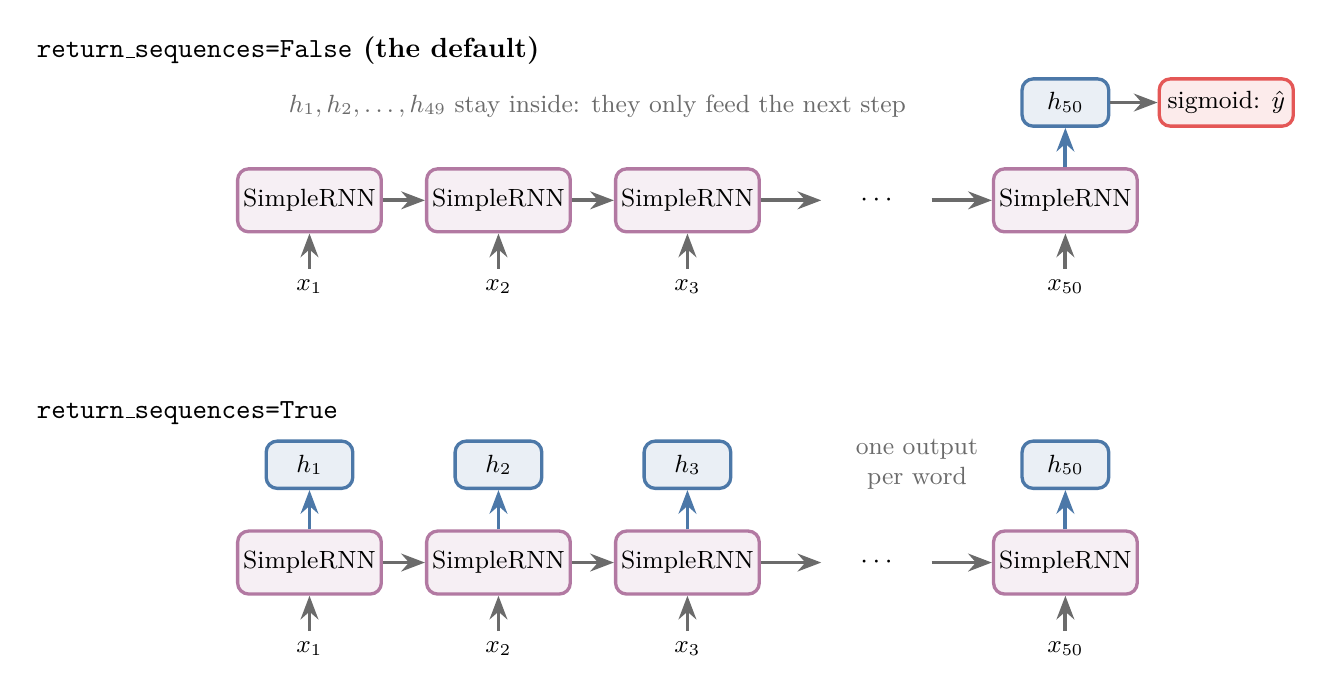
\begin{tikzpicture}[r/.style={box=cpurple, minimum width=1.5cm, minimum height=0.8cm, inner sep=2pt, font=\sffamily\small},
                    inp/.style={font=\sffamily\small}, h/.style={box=cblue, minimum width=1.1cm, minimum height=0.6cm, inner sep=2pt, font=\sffamily\small}]
  \foreach \row/\y/\title in {0/0/{\texttt{return\_sequences=False} (the default)}, 1/-4.6/{\texttt{return\_sequences=True}}} {
    \node[title, anchor=west, font=\sffamily\bfseries] at (-1.2, \y+1.9) {\title};
    \foreach \t/\w [count=\i] in {1/{$x_1$}, 2/{$x_2$}, 3/{$x_3$}, 50/{...}} {
      \ifnum\i=4 \node at (\i*2.4, \y) {$\cdots$};
      \else \node[r] (c\row\i) at (\i*2.4, \y) {SimpleRNN};
            \node[inp, below=0.45cm of c\row\i] (in\row\i) {\w};
            \draw[arrow] (in\row\i) -- (c\row\i);\fi
    }
    \node[r] (c\row5) at (12, \y) {SimpleRNN};
    \node[inp, below=0.45cm of c\row5] (in\row5) {$x_{50}$};
    \draw[arrow] (in\row5) -- (c\row5);
    \draw[arrow] (c\row1) -- (c\row2); \draw[arrow] (c\row2) -- (c\row3); \draw[arrow] (c\row3) -- (8.9, \y); \draw[arrow] (10.3, \y) -- (c\row5);
  }
  % False: only h_50 leaves
  \node[h, above=0.5cm of c05] (o) {$h_{50}$}; \draw[arrow, draw=cblue] (c05) -- (o);
  \node[box=cred, right=0.6cm of o, minimum height=0.6cm, inner sep=3pt, font=\sffamily\small] (y) {sigmoid: $\hat{y}$}; \draw[arrow] (o) -- (y);
  \node[note, anchor=west] at (2.0, 1.2) {$h_1, h_2, \dots, h_{49}$ stay inside: they only feed the next step};
  % True: every h_t leaves
  \foreach \i/\k in {1/1, 2/2, 3/3, 5/50} {\node[h, above=0.5cm of c1\i] (o\i) {$h_{\k}$}; \draw[arrow, draw=cblue] (c1\i) -- (o\i);}
  \node[note, anchor=west] at (9.2, -3.35) {one output\\per word};
\end{tikzpicture}
\end{document}
